\subsection{Lösungsunabhängige Beobachtungen} 
\label{sec:beobachtungen}

Um die Aufgabe zu lösen und einen schnellen Algorithmus zu implementieren wird sich hier zunächst mit einigen wichtigen Beobachtungen auseinandergesetzt, welche essentiell sind um den folgenden Algorithmus zu verstehen.

Ein Tor besteht immer aus einer geraden Strecke. Diese Punkte entsprechen den Pfosten des Tors. Beim Durchschießen eines Tors liegt stets einer der Pfosten links vom Schusspfad und der andere rechts davon, welcher Pfosten links und welcher rechts ist, hängt von der Richtung ab mit der durch das Tor geschossen wird. Diese Konfiguration der linken und rechten Pfosten – die sogenannte \emph{lr-Konfiguration} – gibt also die Schussrichtung des Tors an und umgekehrt.

Bei jeder Aufgabe ist es das Ziel, vom ersten zum letzten Tor zu schießen. Das erste Tor wird im Folgenden als \(t_0\) und das letzte als \(t_n\) bezeichnet. Die Linie, die den linken Pfosten von \(t_0\) mit dem linken Pfosten von \(t_n\) verbindet, wird als \(ll\) benannt, da beide linke Pfosten miteinander verbunden sind. Analog entsteht durch die Verbindung der rechten Pfosten von \(t_0\) und \(t_n\) die Linie \(rr\). Die Tore \(t_0\) und \(t_n\) bilden zusammen mit den Linien \(ll\) und \(rr\) ein Viereck – das \emph{initiale Viereck} (\hyperref[fig:Initialviereck]{Abb. 2}).

\begin{figure}[h]
\label{fig:Initialviereck}
\centering
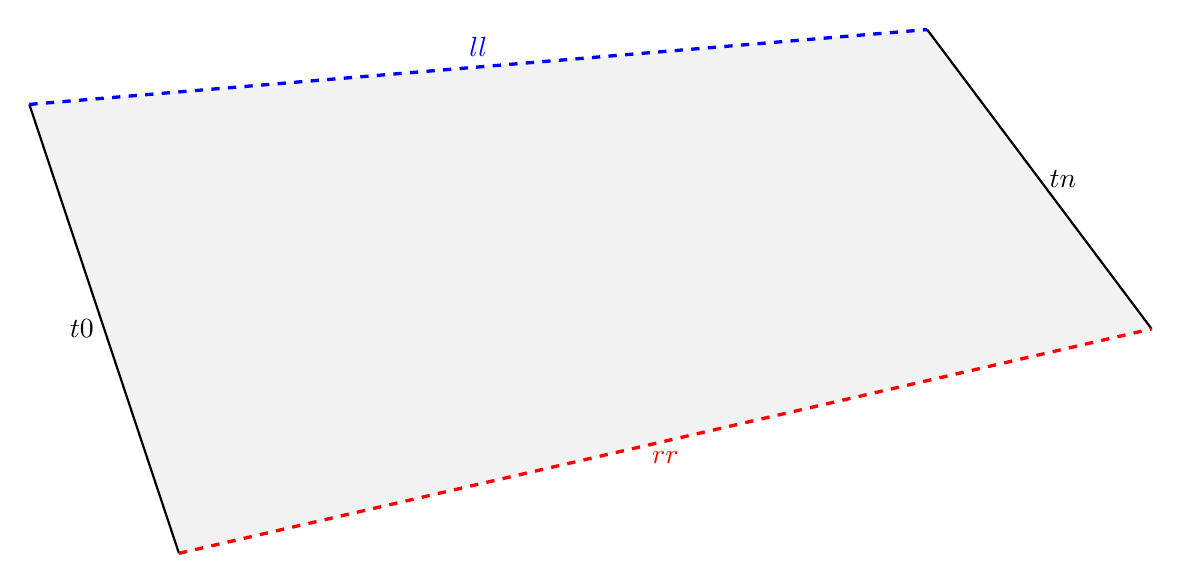
\begin{tikzpicture}[scale=1.9]

	\coordinate (t0L) at (0,2);   
	\coordinate (t0R) at (1,-1);  
	\coordinate (tnL) at (6,2.5);  
	\coordinate (tnR) at (7.5,0.5);  
	

	\fill[gray!10] (t0L) -- (t0R) -- (tnR) -- (tnL) -- cycle;
	
	\draw[thick] (t0L) -- (t0R) node[left, midway] {\(t0\)};
	\draw[thick] (tnL) -- (tnR) node[right, midway] {\(tn\)};
	
	\draw[dashed, blue, very thick] (t0L) -- (tnL) node[above, midway] {\(ll\)};
	\draw[dashed, red, very thick] (t0R) -- (tnR) node[below, midway] {\(rr\)};
	
\end{tikzpicture}
\caption{Initialviereck bestehend aus dem ersten Tor \(t_0\) und dem letzten Tor \(t_n\). Die linken und rechten Pfosten sind jeweils mit einer Linie \(ll\) bzw. \(rr\) verbunden. Jede mögliche Lösung muss durch dieses Initialviereck laufen.}

\end{figure}


Das Initialviereck, bestehend aus \(t_0\), \(t_n\), \(ll\) und \(rr\), stellt einen Kanal dar, durch den jeder mögliche Schuss verlaufen muss. Ist die lr-Konfiguration für jedes Tor bekannt, lässt sich ein \emph{Kanalpolygon} (\hyperref[fig:kanalpolygon]{Abb. 3a und 3b}) konstruieren, indem alle linken und rechten Pfosten in der richtigen Reihenfolge miteinander verbunden werden. Wenn sich die Verbindungsstrecken des Kanalpolygons überkreuzen, so ist die Aufgabe nicht lösbar, da die Tore entweder in der falschen Reihenfolge angeordnet sind oder kein Pfad durch das Kanalpolygon mehr führt. Daher muss zunächst überprüft werden, ob ein valides Kanalpolygon existiert.




\begin{figure}[t]
    \centering

    \vspace{-1cm} 
    \begin{subfigure}{\linewidth}
        \centering
        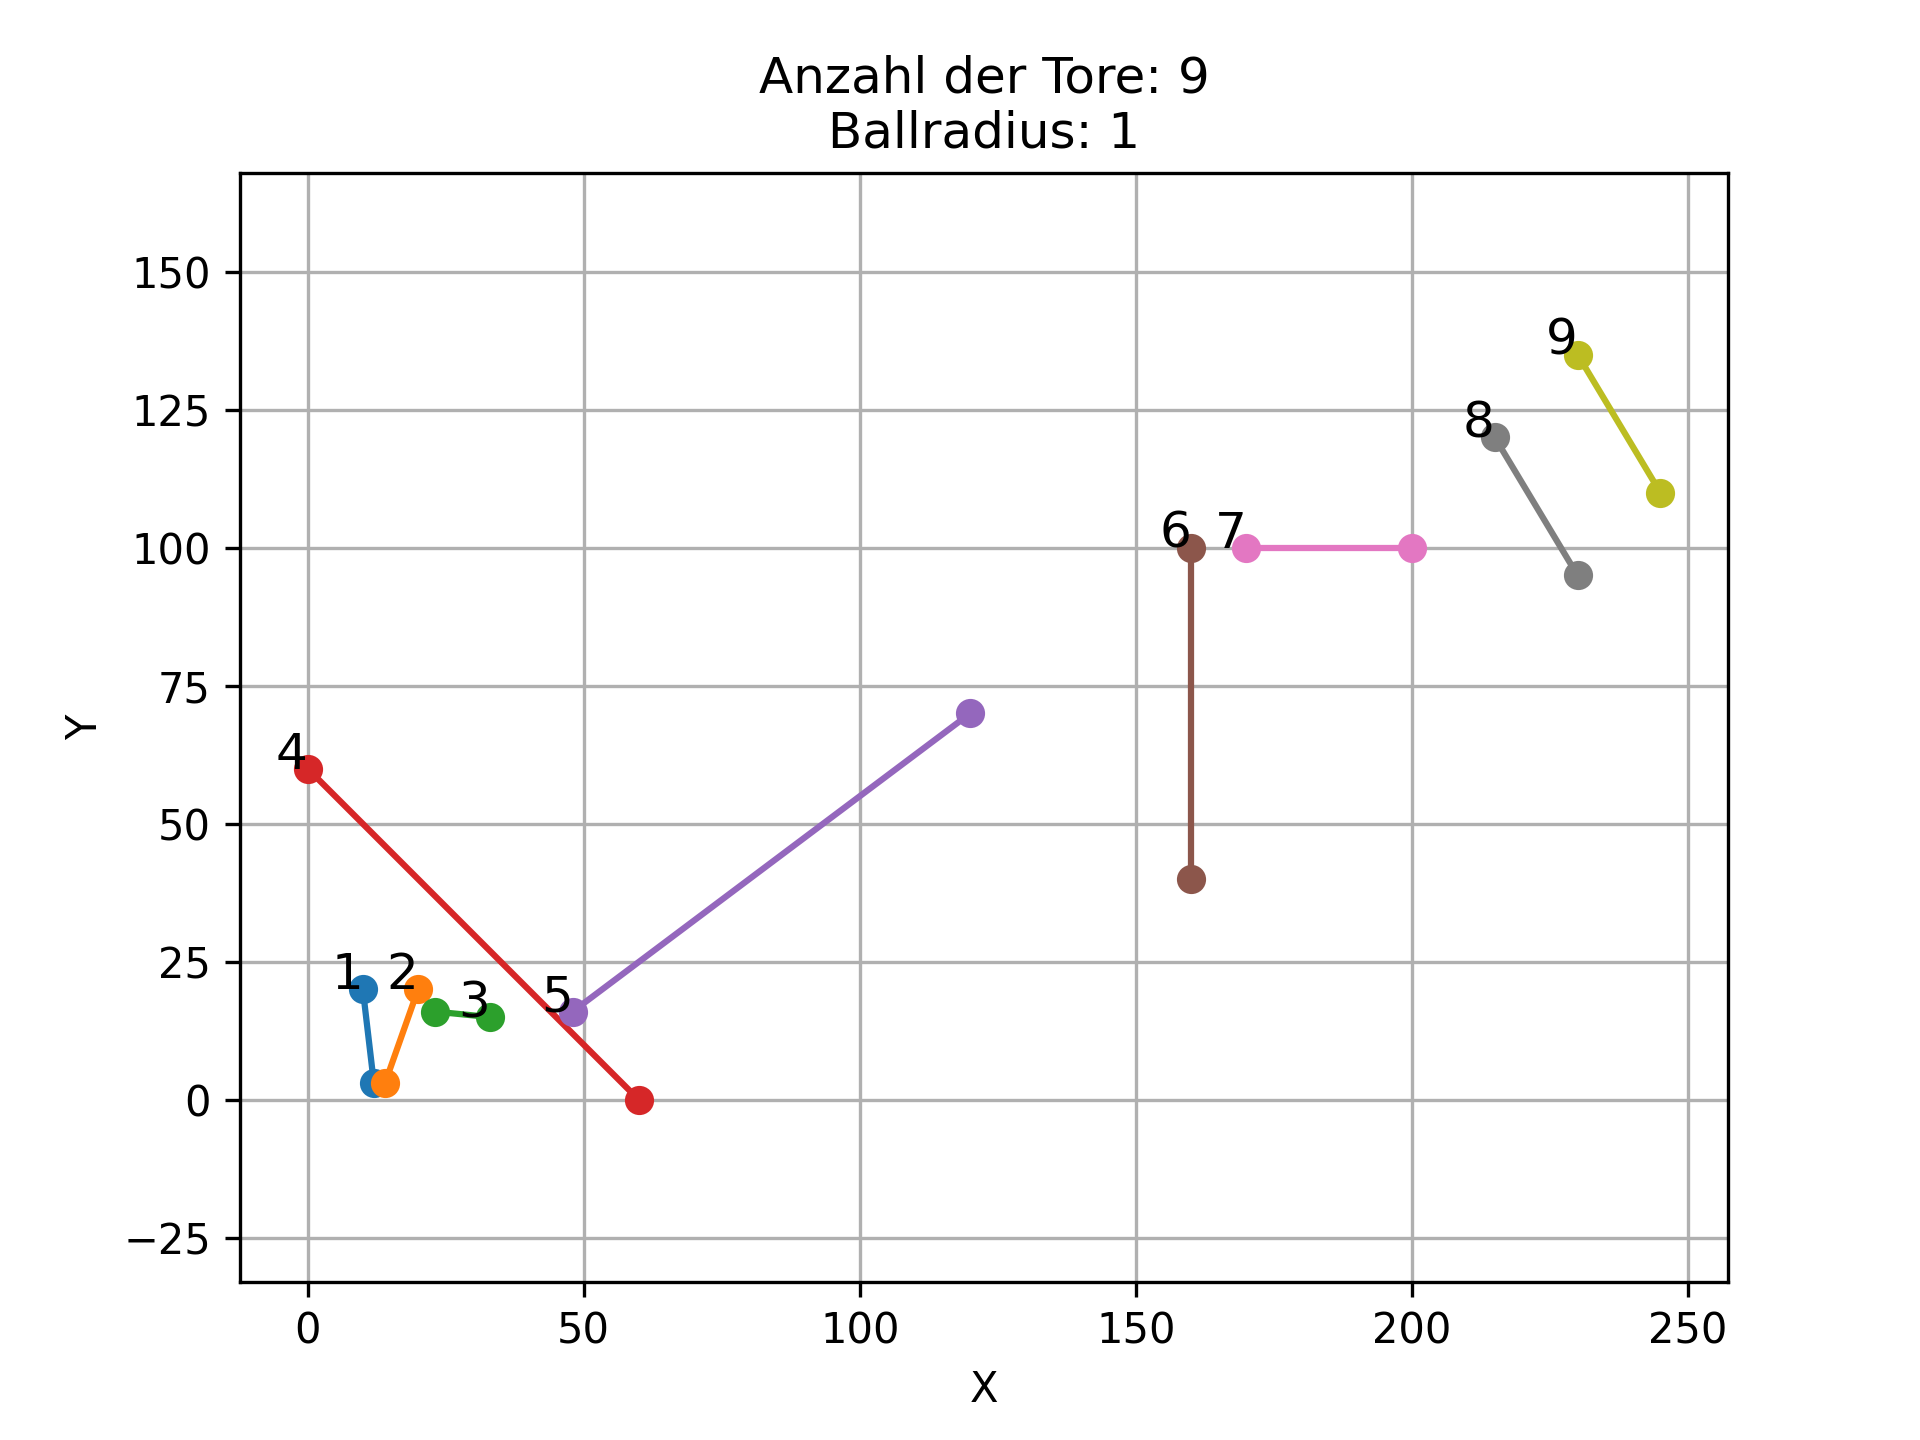
\includegraphics[width=0.8\linewidth]{images/krocket1.png}
        \caption{}
        \label{fig:tore}
    \end{subfigure}
    \vspace{-0.5cm}        

    \begin{subfigure}{\linewidth}
        \centering
        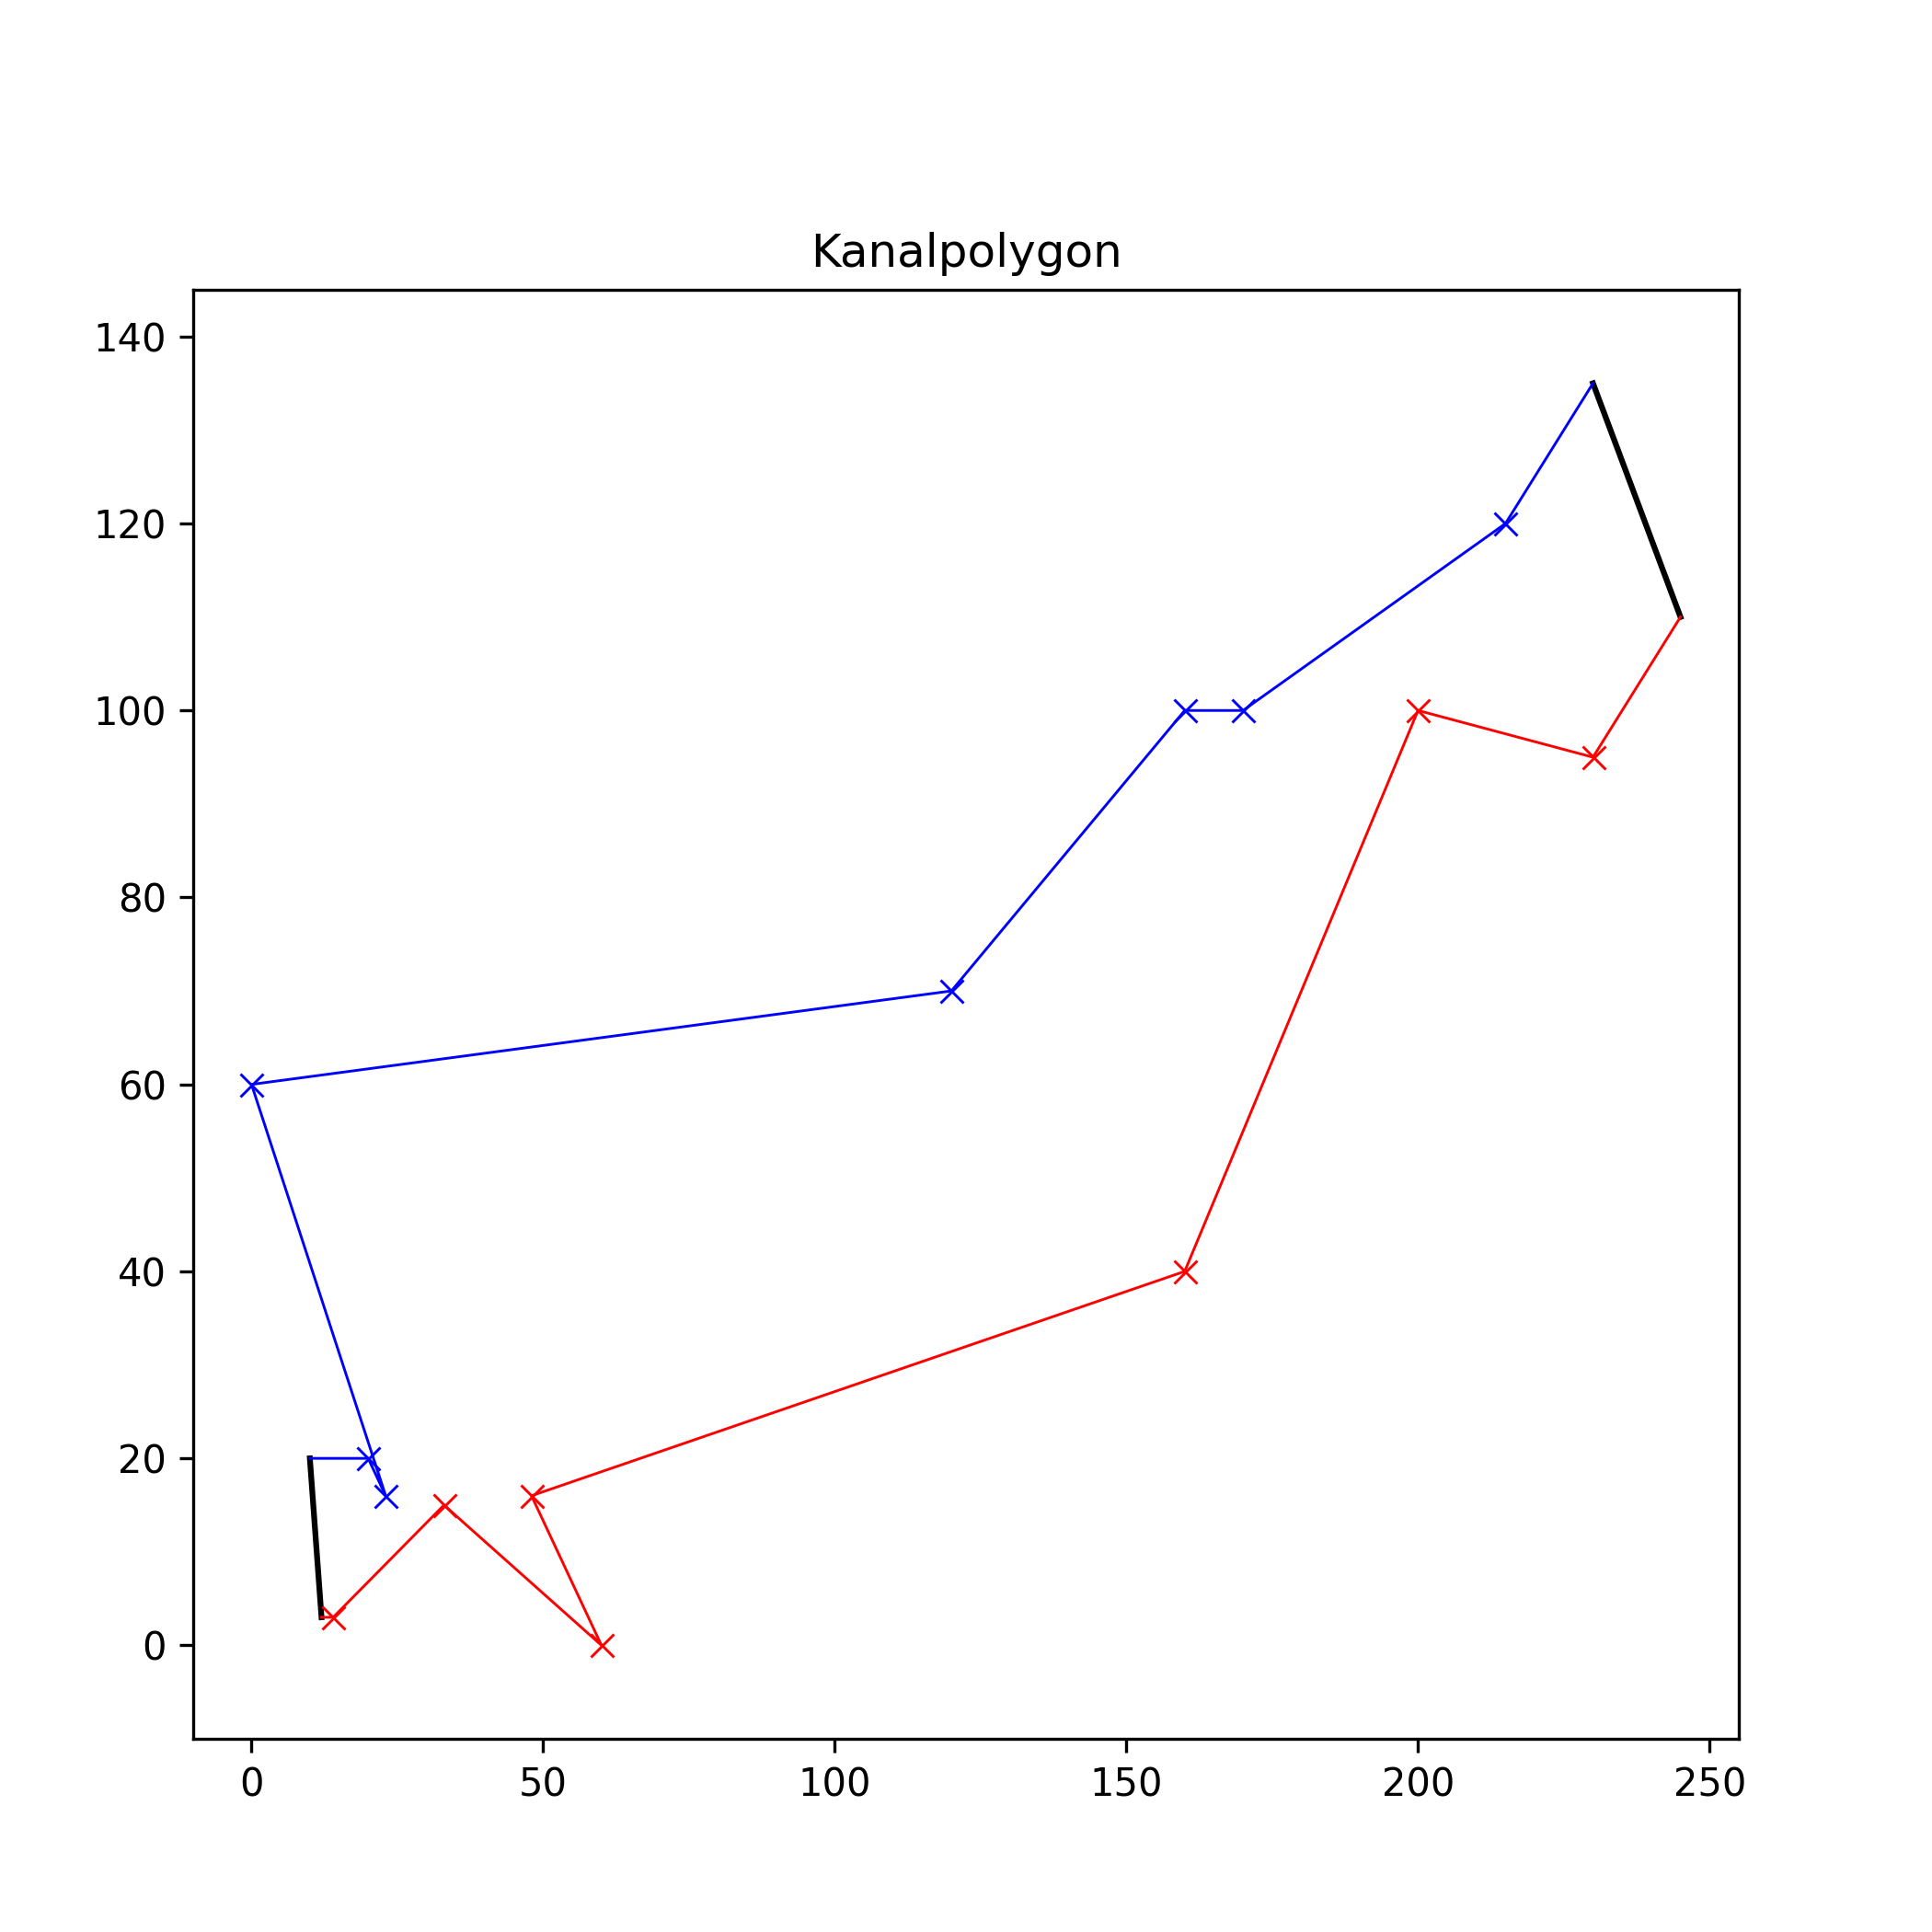
\includegraphics[width=0.8\linewidth]{images/testplot.png}
        \caption{}
        \label{fig:kanalpolygon}
    \end{subfigure}

    \caption{Vergleich zwischen Beispielaufgabe und Kanalpolygon. In Grafik (a) ist die Beispielaufgabe 1 aus dem 43. Bundeswettbewerb Informatik abgebildet. Alle Tore sind nummeriert und in unterschiedlichen Farben dargestellt. Aus dieser Aufgabe wird das Kanalpolygon in Grafik (b) erstellt, indem alle linken Pfosten (blau) und alle rechten Pfosten (rot) miteinander verbunden werden. Das erste Tor \(t_0\) und das letzte Tor \(t_n\) sind als schwarze Linien dargestellt.}
\end{figure}
